\section{Results and evaluation} \label{sec:results}

\subsection{Overview of datasets and hardware used for testing}
\label{sec:overview_of_datasets}

A couple of different datasets will be used for testing and evaluating the
implementation of the distance metrics and clustering algorithms presented in
section \ref{sec:methods}. These datasets will be briefly presented in this
section.

\begin{description}
  \item[\texttt{SILVA}] \hfill \\
    The dataset \texttt{SILVA\_119\_SSURef\_tax\_silva.fasta} has a size of
    around 2.3 GB and contains \num{1583830} RNA sequences.

  \item[\texttt{RDP}] \hfill \\
    The dataset \texttt{RDP\_Pro\_Full.sort.fna} has a size of around 3.5 GB
    and contains \num{3019928} DNA sequences.
\end{description}

Various statistics about the datasets are shown in Table \ref{tab:data_stats}.
The error ratio is the ratio between the number of non DNA/RNA bases, i.e. the
ambigious bases.

\begin{table}[H]
  \centering
  \begin{tabular}{c | c | c | c | c | c}
    Dataset        & Avg. len. & Min. len. & Max. len. & Median len. & Error ratio \\
    \hline\hline
    \texttt{SILVA} & \num{1415.46}  & \num{900} & \num{3845} & \num{1389}       & 0.000156146 \\
    \texttt{RDP}   & \num{1044.19}  & \num{400} & \num{2922} & \num{1132}       & 0.000798764 \\
  \end{tabular}
  \caption{Various information about the different datasets.}
  \label{tab:data_stats}
\end{table}

The hardware used for testing was a 64-bit Intel Core i5-2520M 2nd generation
Sandy Bridge processor with a base frequency of 2.5 GHz and with 2 cores (4
hardware threads), and 16 GB RAM.


\subsection{Testing the distance metric on altered sequences}
\label{sec:altered_sequences}

Two different sets of highly similar sequences was constructed from a real
world sequence from \texttt{SILVA} and this was used in the evaluation of the
distance metric.

One sequence was chosen, 10 copies of this sequences were made and to each of
these copies, a few alterations were made. In the first set, a list of random
indices in the sequence were generated and in each of these indices in the
sequence, a substitution for a different, randomly chosen nucleotide was made.
This was done twice, for different degrees of alteration, and the number of
alterations was equal to respectively 1\% and 2\% of the length of the
sequence.

In the second set, the same number of alterations to individual nucleotides
were made, but in this case they were grouped into alterations of substrings of
length 5 (one such group being of length less than 5 if the number of
alterations was not a multiple of 5).

For illustration, Figure \ref{fig:alterations} shows an original sequence in
the first line, the single edits alterated sequence in the second line and the
chunk alterated sequence in the third line.

\newcommand{\tc}[1]{\textcolor{red}{#1}}
\begin{figure}[H]
  \centering
  \texttt{AAAAAAAAAAAAAAAAAAAAAA} \\
  \texttt{AAAAA\tc{T}AA\tc{C}AAAA\tc{G}AAAA\tc{T}AAA} \\
  \texttt{AAA\tc{TC}AAAAAAAAAA\tc{GG}AAAAA}
  \caption{Two types of alterations to sequences: the original sequence in the
    first line, single edit alterations in the second line and chunks of edits
    in the third line.}
  \label{fig:alterations}
\end{figure}

The $k$-mer based distance metric, presented in section
\ref{sec:kmer_distance}, is expected to be more sensitive to a number of
individual changes than to the same number of changes made in chunks. This test
serves to confirm this expectation and to give an insight into the change in
$k$-mer distance when performing a controlled number of edits.

The similarities between the original sequence from \texttt{SILVA} and the 10
altered sequences, for the four different types of alterations, are shown in
Table \ref{tab:altered_seqs_similarities}.

\begin{table}[H]
  \centering
  \begin{tabular}{c|c||c|c}
    \multicolumn{2}{c||}{single edits}  & \multicolumn{2}{c}{chunk edits} \\
    \hline\hline
    1\%   &   2\%                   &   1\%   &   2\% \\
    \hline
    0.944   & 0.889                     & 0.980     & 0.960 \\
    0.947   & 0.887                     & 0.979     & 0.960 \\
    0.944   & 0.893                     & 0.979     & 0.960 \\
    0.941   & 0.902                     & 0.979     & 0.961 \\
    0.944   & 0.894                     & 0.979     & 0.958 \\
    0.947   & 0.894                     & 0.979     & 0.958 \\
    0.941   & 0.895                     & 0.982     & 0.958 \\
    0.945   & 0.891                     & 0.979     & 0.961 \\
    0.945   & 0.889                     & 0.979     & 0.958 \\
    0.946   & 0.897                     & 0.981     & 0.958
  \end{tabular}
  \caption{Similarity measures, using $k=6$, for 1\% and 2\% single edits,
    respectively, and 1\% and 2\% chunk edits, respectively, to 10 copies of a
    single sequence.}
  \label{tab:altered_seqs_similarities}
\end{table}

As expected, the single edits result in a lower similarity that the
corresponding chunk edits. This is because five individual changes will affect
the count of up to $5 \cdot k$ $k$-mers, while five changes in sequence will
only affect up to $4+k$ $k$-mers.


\subsection{Comparing \textsc{K-Dist} with the Levenshtein distance metric}
\label{sec:kdist_vs_levenshtein}

This section compares the implementation of the \textsc{K-Dist} distance metric
(Algorithm \ref{alg:K-Dist}) with the implementation of the bottom-up dynamic
programming (DP) algorithm (Algorithm \ref{alg:levenshtein} in appendix
\ref{app:levenshtein_algorithm}) for the Levenshtein distance metric.

The data in Table \ref{tab:levenshtein_vs_kdist_performance} shows how many
comparisons per second the implementation of Levenshtein and the implementation
of \textsc{K-Dist} can afford. This is shown for various values for the $k$
parameter. The tests were performed on the \texttt{SILVA} dataset.

\begin{table}[H]
  \centering
  \begin{tabular}{ c | r }
    Distance metric implementation  & Comparisons/second    \\
    \hline \hline
    Levenshtein (DP)                & $\approx \num{195}$   \\ \hline
    \textsc{K-Dist}, $k=4$          & $\approx \num{91500}$ \\ \hline
    \textsc{K-Dist}, $k=5$          & $\approx \num{91000}$ \\ \hline
    \textsc{K-Dist}, $k=6$          & $\approx \num{89000}$ \\ \hline
    \textsc{K-Dist}, $k=7$          & $\approx \num{72500}$ \\ \hline
    \textsc{K-Dist}, $k=8$          & $\approx \num{46000}$ \\
  \end{tabular}
  \caption{Performance comparison between the bottom-up, dynamic programming
    Levenshtein implementation and \textsc{K-Dist} implementation with
    different values for the $k$ parameter. Tested with the \texttt{SILVA}
    dataset.}
  \label{tab:levenshtein_vs_kdist_performance}
\end{table}

The \textsc{K-Dist} implementation with $k=4$ is more than 460 times faster
than the Levenshtein implementation, but becomes slower with increasing values
for $k$, with the \textsc{K-Dist} implementation being around 235 times faster
for $k=8$.

As mentioned in section \ref{sec:edit_distance}, the running time of the
presented Levenshtein algorithm is near quadratic in the lengths of the
strings, while the running time of the \textsc{K-Dist} algorithm is
$\Theta(\max{(\abs{s},\abs{t})}-k)$, where $s$ and $t$ are the sequences being
compared and $k$ is the value for the parameter $k$. This was analyzed in
section \ref{sec:k-dist_analysis}. So \textsc{K-Dist} will always be faster
that the presented algorithm for Levenshtein for long enough sequences and as
shown above in Figure \ref{tab:levenshtein_vs_kdist_performance}, that is
indeed the case for the sequences this project is concerned with.

Scatter plots of \textsc{K-Dist} similarities and the corresponding Levenshtein
similarities for parameters $k=5$ and $k=8$ are shown in Figure
\ref{fig:k-dist_lev_similarity_k5} and Figure
\ref{fig:k-dist_lev_similarity_k8}, respectively. These similarity measures
have been obtained by comparing the 500 first sequences from \texttt{SILVA}
with each other.

Since the Levenshtein distance does not produce values between 0 and 1, a
similarity ratio similar to the one used in \textsc{K-Dist} and expressed in
equation (\ref{eq:Manhattan_similarity}) was used. Specifically, the ratio
between the Levenshtein distance and the maximum possible distance subtracted
from one. The maximum possible Levenshtein distance is equal to the length of
the longer sequence.

\begin{wrapfigure}{l}{0.55\textwidth}
  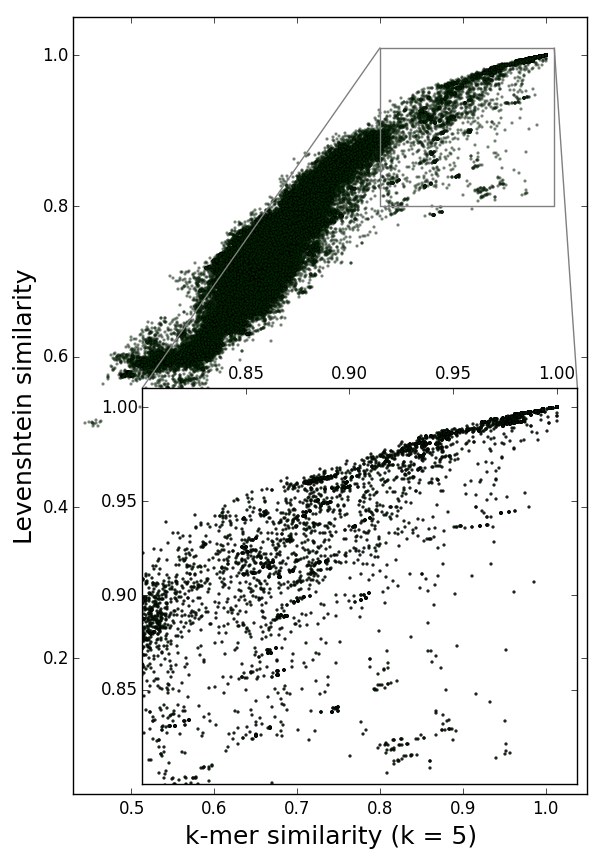
\includegraphics[width=0.55\textwidth]{graphics/Levenshtein_K-Dist_k5.png}
  \caption{Scatter plot comparison of similarity measures for Levenshtein and
    \textsc{K-Dist} with $k=5$ on the first 500 sequences of \texttt{SILVA}.}
  \label{fig:k-dist_lev_similarity_k5}
\end{wrapfigure}

As seen in the figures, there is a monotonically increasing relationship
between the two similarity metrics. Additionally, the Levenshtein similarities
barely get below 0.5, while the interval of the \textsc{K-Dist} similarities is
around $[0.4,1.0]$ for $k=5$ and $[0,1]$ for $k=8$. This is likely because the
number of different 8-mers is much greater than the number of different 5-mers,
so it is less likely that two $k$-mers are the same. That will result in a
greater distance and hence a lower similarity.

Since transposable elements will not result in much decrease in similarity for
\textsc{K-Dist}, but will do so for Levenshtein, there will be some measures
which are relatively lower for Levenshtein than for \textsc{K-Dist}. The
``width'' of the points in Figure \ref{fig:k-dist_lev_similarity_k5} and
\ref{fig:k-dist_lev_similarity_k8} can likely be partly attributed to this
difference in characteristic between the two distance metrics.

The subplots, i.e. the inner boxes, in Figure
\ref{fig:k-dist_lev_similarity_k5} and \ref{fig:k-dist_lev_similarity_k8},
shows a zommed in view of the parts of the scatter plots that lies in the
interval $[0.8,1.0]$ on both axes. The most interesting Levenshtein
similarities are those above or equal to $0.95$. These points lie fairly high
for the corresponding \textsc{K-Dist} similarity, for the most part, i.e. the
majority of the comparisons that give a Levenshtein similarity of $0.95$ also
gives a \textsc{K-Dist} similarity of $0.85$ or above.

\begin{figure}[H]
  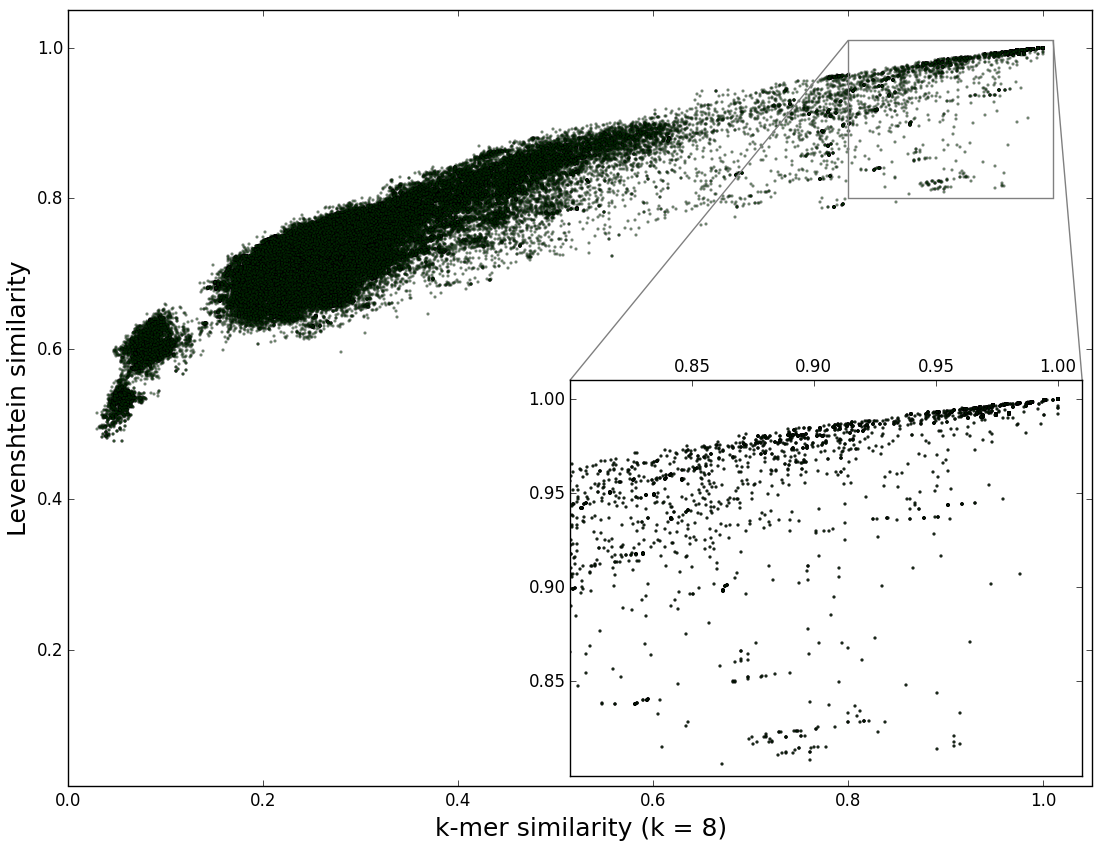
\includegraphics[width=1.0\textwidth]{graphics/Levenshtein_K-Dist_k8.png}
  \caption{Scatter plot comparison of similarity measures for Levenshtein and
    \textsc{K-Dist} with $k=8$ on the first 500 sequences of \texttt{SILVA}.}
  \label{fig:k-dist_lev_similarity_k8}
\end{figure}


\subsection{Evaluating \textsc{K-Clust} on a synthetic dataset}
\label{sec:synth_dataset}

A synthetic dataset was constructed for evaluating the \textsc{K-Clust}
algorithm's ability to find the right clusters in a dataset with a clearly
correct, expected clustering result.

A set of $380$ sequences with mutual similarities of at most $0.6$ was
extracted from \texttt{SILVA}, using the \textsc{K-Dist} distance metric
(Algorithm \ref{alg:K-Dist}) with parameter $k=5$. For each of these
sequences, $999$ copies were made and chunks of changes were made to these as
described above in section \ref{sec:altered_sequences}, corresponding to $2$\%
of the characters of each sequence. This yields a set of \num{380000}
sequences with $380$ expected clusters, which each should contain sequences
with similarities of approximately $0.92$ since all sequences are changed and
a $2$\% change to a sequence gives an average similarity from the original
sequence of around $0.96$, cf. section \ref{sec:altered_sequences}.

The sequences expected to be in the same cluster was given the same description
in the \texttt{FASTA} file, i.e. the same text string after ``>'', to make it
easy to evaluate the result from the clustering. Furthermore, the sequences
were placed in random order before running \texttt{klust} on the data.

The synthetic dataset was made fairly large, both in number of sequences and in
number of expected clusters, to be able to properly test the clustering
algorithm's ability to search for the correct centroid and not stop the search
prematurely which would result in a new cluster being created and a different
clustering result than the expected one.

As hoped, running \texttt{klust} on the constructed dataset, with parameters
$k=5$, $id=0.85$ and $max\_rejects=8$ gives a clustering output consisting of
$380$ clusters with 1000 sequences in each (including the centroid). The
terminal output from the program is shown in Figure
\ref{fig:synth_silva_output} in appendix \ref{app:synth_dataset} and an
excerpt from the clustering ouput file created by the program is shown in
Figure \ref{fig:synth_silva_clustering} in the same appendix. This shows that
the sequences in each cluster have the same description line, i.e. they were
constructed to be similar and should indeed be in the same cluster. The result
was equally correct when clustering with a threshold parameter of $0.89$, but
the results start containing a few errors when clustering with a threshold of
$0.9$ or above. In the specific test, and the specific, random order of the
sequences, the clustering result yielded $386$ clusters for $id=0.9$, average
cluster size of $984.456$ and a minimum cluster size of $33$.

This test provides some evidence that \textsc{K-Clust} is able to successfully
cluster a dataset of a fairly realistic size. Since the similarities are known
a priori and the cluster sequences are constructed to be of a similarity around
$0.92$ on $k=5$, this is not a test of the \textsc{K-Dist} distance metric.


\subsubsection{Multidimensional scaling of the synthetic dataset}
\label{sec:mds_synth}

\emph{Multidimensional scaling} (MDS) of the sequences in the synthetic dataset
was used to visualize and further evaluate the clustering result from the
previous section (section \ref{sec:synth_dataset}). Multidimensional scaling is
used to visualize the distances between all the sequences in the synthetic
dataset in two dimensions, i.e. a scatter plot that tries to maintain the
relative distances between the sequences as well as possible.

The technique used for dimensionality reduction was \emph{t-distributed
Stochastic Neighbor Embedding} (t-SNE)~\cite{maaten}. This was done using
\texttt{Python} with \texttt{matplotlib} and \texttt{scikit-learn}. Sequences
expected to be in the same cluster were given the same color and thus the MDS
is expected to give a visualization of separate clusters of points of the same
color. Centroids were given a cirle marker and all other sequences were gives a
``+'' marker.

A subset of the synthetic set described in section \ref{sec:synth_dataset} was
used for the MDS, because the scatter plot easily becomes too densely
populated and because the computation is too expensive for \num{380000}
sequences. A set of $400$ sequences, consisting of $40$ expected clusters with
$10$ sequences in each, was used for the visualization shown in Figure
\ref{fig:mds_synth}. The clustering indicated by the colors and markers is
from \textsc{K-Clust} and the distances used for MDS are calculated using
\textsc{K-Dist}.

\begin{figure}[h!]
  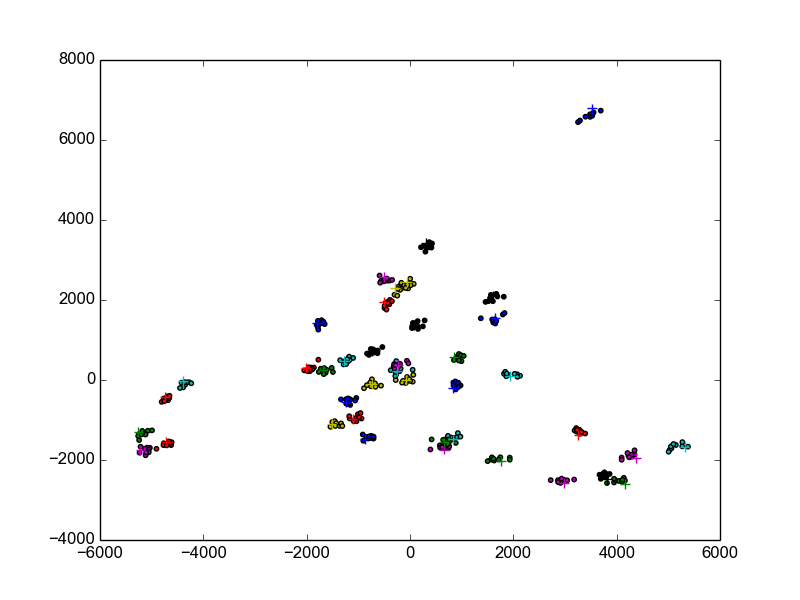
\includegraphics[width=\textwidth]{graphics/MDS_t-SNE_synth_silva_400.png}
  \caption{Multidimensional scaling using t-SNE of the 400 sequences and
    40 expected clusters from the synthetic dataset described in section
    \ref{sec:synth_dataset}. The distances are calculated using
    \textsc{K-Dist}. The clustering result from \texttt{klust} with $k=5$,
    $id=0.85$ and $max\_rejects=8$ is used to color different clusters with
    different colors. Centroids are marked with a circle and non-centroid
    sequences with a ``+''.}
  \label{fig:mds_synth}
\end{figure}

The results from \texttt{klust} on the synthetic dataset was correct and
completely as it was constructed to be. Similarly, the MDS in figure
\ref{fig:mds_synth} shows a very clear set of clusters of points, of distinct
colors, marked with ``+'' symbols and a single centroid for each cluster, which
is marked with a circle with the same color in the middle. There are only small
errors such as single sequences lying a bit away from their respective clusters
and very closely positioned clusters. However, this might easily have to do
with the actual MDS visualization of the data, since MDS does not provide a
perfect two-dimensional version of the high-dimensional distances.

Figure \ref{fig:mds_synth_lev} shows the same clustering result as in Figure
\ref{fig:mds_synth}, i.e. the same coloring and marking, but with the distances
for the MDS calculated using Levenshtein. This provides even some more insight
into the relationship between \textsc{K-Dist} and Levenshtein, and helps to
verify the suitability of \textsc{K-Dist} as an approximation for sequence
similarity, given that Levenshtein measure the actual edit distance.

\begin{figure}[h!]
  \centering
  \def\svgwidth{\columnwidth}
  \import{graphics/}{MDS_Levenshtein.pdf_tex}
  \caption{Multidimensional scaling using t-SNE of the 400 sequences and 40
    expected clusters from the synthetic dataset using Levenshtein distance.
    The clustering result from \texttt{klust} with $k=5$, $id=0.85$ and
    $max\_rejects=8$ is used to color different clusters with different
    colors. Centroids are marked with a circle and non-centroid sequences
    with a ``+''.}
  \label{fig:mds_synth_lev}
\end{figure}

Once again, the results look very clear and as hoped, but there does seem to be
a little more overlap in the clusters, although this might again be partly
attributed to the imperfection of MDS. In any case, the clusters are also very
apparent when using the Levenshtein distance measure and this indicates that
the $k$-mer based \textsc{K-Dist} functions properly as an approximation of
distance. Specifically, the colors are not mixed up so it is not the case that
one similarity metric gives a very low similarity while the other gives a very
high similarity, and vice versa, for some sequences.


\subsection{Evaluating \textsc{K-Clust} on real data using MDS}
\label{sec:mds_real_data}

The \textsc{K-Clust} algorithm was also tested on real data, specifically the
first 500 sequences of the \texttt{SILVA} dataset, using MDS to visualize the
sequence similarities and the clustering result, as described in section
\ref{sec:mds_synth}.

\begin{figure}[H]
  \centering
  \begin{subfigure}[t]{1.0\textwidth}
    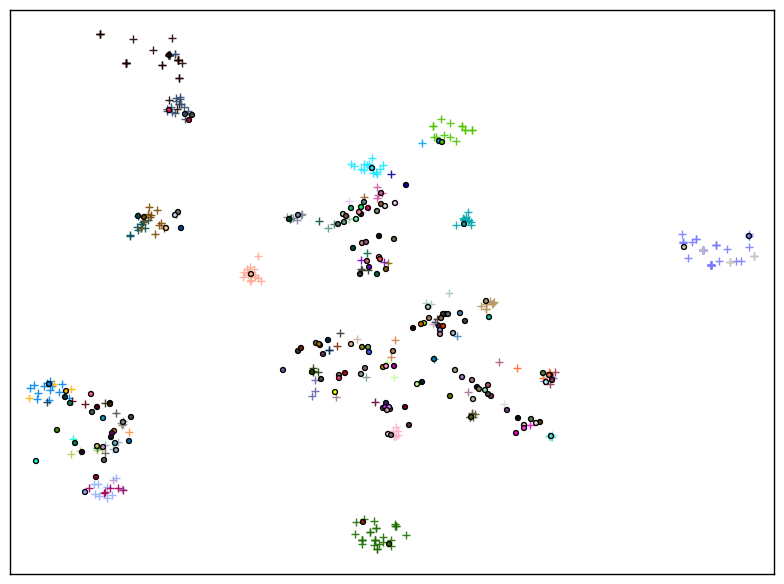
\includegraphics[width=1.0\textwidth]{graphics/SILVA_t-SNE_500.png}
    \caption{Sequences not sorted.}
    \label{fig:mds_silva_no_sort}
  \end{subfigure}

  \hfill\\
  \hspace{2em}
  \begin{subfigure}[b]{1.0\textwidth}
    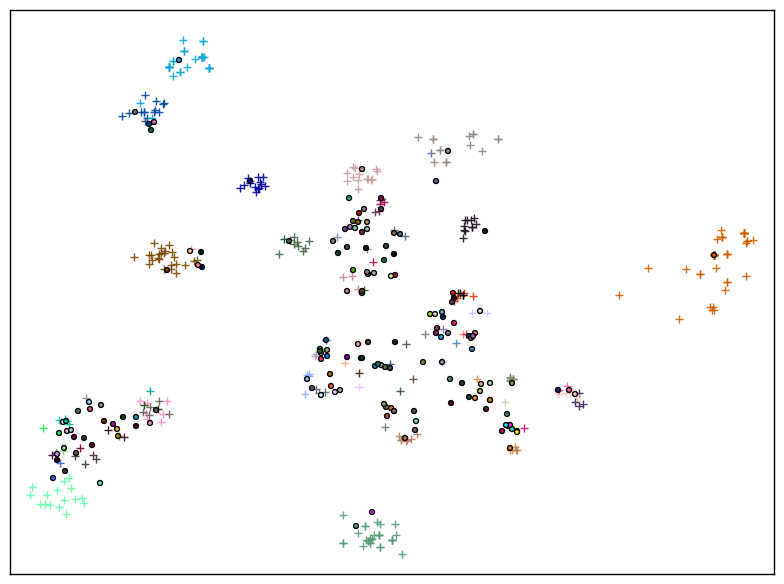
\includegraphics[width=1.0\textwidth]{graphics/SILVA_t-SNE_incr_sort_500.png}
    \caption{Sorted by increasing sequence length.}
    \label{fig:mds_silva_sort_incr}
  \end{subfigure}
\end{figure}
\clearpage
\begin{figure}[H]
  \ContinuedFloat
  \begin{subfigure}[b]{1.0\textwidth}
    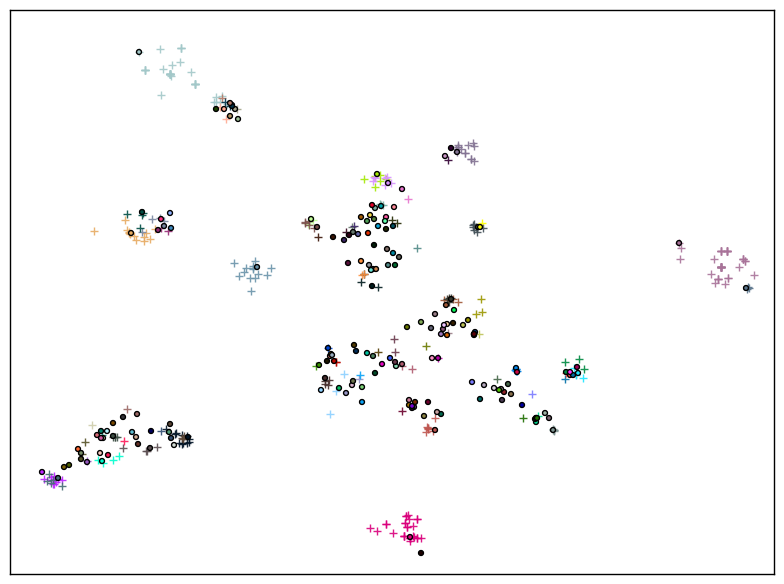
\includegraphics[width=1.0\textwidth]{graphics/SILVA_t-SNE_decr_sort_500.png}
    \caption{Sorted by decreasing sequence length.}
    \label{fig:mds_silva_sort_decr}
  \end{subfigure}
  \caption{MDS using t-SNE of the first 500 sequences from \texttt{SILVA} with
    the clustering result from \texttt{klust}, using parameters $k=5$,
    $id=0.85$ and $max\_rejects=8$, used to color different clusters with
    different colors. Centroids are marked with a circle. Sequences were sorted
    by length before clustering as noted under each subfigure.}
  \label{fig:mds_silva}
\end{figure}

The clustering result from \texttt{klust} on \texttt{SILVA} consists of
clusters of very different sizes and a large number of singleton clusters, i.e.
clusters containing only the centroid sequence. This means that this data will
be harder to visualize nicely with MDS, since the sequences will not be as
clearly partitioned into a few clusters of the same size. However, it should at
least be possible to identify the sequences of large clusters and observe
whether they are indeed close to each other in the MDS.

Figure \ref{fig:mds_silva} (\subref{fig:mds_silva_no_sort}),
(\subref{fig:mds_silva_sort_incr}) and (\subref{fig:mds_silva_sort_decr}) shows
MDS of the first 500 sequences from \texttt{SILVA}, with the sequences not
sorted, sorted by increasing length and sorted by decreasing length,
respectively, before clustering with \texttt{klust}.

Both respectively, shows a few apparent clusters, but as expected they also
show a large number of smaller clusters and singleton clusters. In this
particular example, when running \texttt{klust} with parameters $k=5$,
$id=0.85$ and $max\_rejects=8$, the number of resulting clusters were $159$ with
a maximum cluster size of $38$, average size approximately \num{3.145}.
Furthermore, the result contained $87$ singleton clusters.

The large number of singleton clusters and small clusters are especially
apparent in the center of the figures and in the lower left part of the
figures. Since the number of clusters is so high, it is likely that the MDS
causes the sequences to be more crammed togetether and apear more dense than
if the number of clusters had been lower.

% TODO: more discussion


\subsection{Evaluation of centroid search in \texttt{klust}}
\label{sec:evaluation_centroid_search}

A great part of the clustering lies in task of locating potential matching
centroids to a sequence. To evaluate this, \texttt{klust} was run on a number
of sequences from the dataset \texttt{SILVA}. Information about how many times
an actual comparison was made and scored under the similarity threshold was
extracted. False negatives were also extracted, i.e. how often a comparison
was not made, but it would have scored over the similarity threshold. How
often it performs a comparison against how often it does not and how often it
reaches the $max\_reject$ parameter was also measured. Table
\ref{tab:centroid_search_data} show this data represented as ratios. The
program was run with parameters $k=5$, $id=0.85$, $max\_rejects=8$ and flag
\texttt{-{}-sort\_incr}.

\begin{table}[H]
  \centering
  \begin{tabular}{c|c|c}
  Count                & \num{10000} & \num{100000} \\
  \hline\hline
  Reject ratio         & 0.00231  & 0.00872 \\
  \hline
  False negative ratio & 0.00048  & 0.00013 \\
  \hline
  Try ratio            & 0.00377  & 0.00112 \\
  \hline
  Reached max rejects  & 0           & 4 \\
  \end{tabular}
  \caption{Data on the first \num{10000} and \num{100000} sequences of 
  \texttt{SILVA} showing reject ratio, how many times a query sequence was 
  compared to a target sequence and falled under the similarity threshold, and 
  a false negative ratio which is how often a sequence was not compared to a 
  target sequence but would have matched it. It also shows a try ratio, how 
  often a query sequence was tried compared to a target sequence, and how many 
  times a query sequence was dismissed because it was rejected too many times.}
  \label{tab:centroid_search_data}
\end{table}

There are very few rejects in both cases, which means the initial check for
the $k$-mer intersection is actually very accurate representation of sequence
similarity. There are more rejects as there are more sequences to be
clustered. This should not be seen as a drawback for the clustering quality.
On the contrary, it means it performs more compares and as a result, the
number of false negatives fall. The only loss, besides making a couple of
additional compares, is that it can reject the same sequence too many times
($max\_rejects$) and make the sequence a centroid without comparing it too
anymore centroids. This is likely because the sequence has many distinct
$k$-mers and thus often match the intersection criteria. These will often not
match the centroids, and while they might match a centroid, without a
$max\_reject$ it can essentially compare to all centroid. This is good to
avoid as it is heavily slows the clustering down.

The try ratio, how often it succeeds in the initial criteria, is quite low and
even falls when clustering more sequences. When clustering \num{100000}
sequences it will only make a comparison every $1$ in $900$ times. This is
quite low and is the primary slow down in the clustering algorithm. Since it
already chooses to perform the comparisons with very little error (small
reject and false negative ratios) the only way to make the clustering faster
is to find the right ones faster. This is the intended optimization a link can
introduce (cf. section \ref{sec:k-clust_algorithm}).


\subsection{Evaluating \texttt{klust} on real data and comparing with
            \texttt{USEARCH}}
\label{sec:evaluating_klust_real_data}

To test the performance and quality of the program, it was run on different
parameters and settings. The table in appendix \ref{app:klust_data_parameters}
shows output data from running the first \num{100000} sequences from
\texttt{SILVA} with different parameters. Sorting by increasing length is on
average $21.65\%$ faster and never slower than not sorting. It is also on
average $42.63\%$ faster and never slower than sorting by decreasing length.
Furthermore, sorting by increasing length on average has $8.77\%$ fewer
clusters and never more clusters than not sorting. It has $25.07\%$ fewer
clusters on average and never more clusters than when sorting by decreasing
length. Generally higher $k$'s are also expected to produce more clusters,
since the comparison punishes mismatches more than lower $k$'s as discussed in
section \ref{sec:altered_sequences}.

The data shows that sorting by increasing length is always preferrable. The
higher $k$'s are also generally much slower and the comparisons are very
strict, i.e. the identity should be lower for the higher $k$. Section
\ref{sec:synth_dataset} and the multidimensional scaling plots in Figure
\ref{fig:mds_synth} and Figure \ref{fig:mds_silva_sort_incr} shows that $k=5$
is a good choice in terms of sensitivity. Another interesting choice is $k=6$,
since it does almost the same comparisons per second (cf. Figure
\ref{tab:levenshtein_vs_kdist_performance}). These results gives the incentive
to study $k=5$ and $k=6$, when sorting by increasing length, further. The
reason lower values of $k$ are not investigated is because the number of
distinct $k$-mers is too low, so the interval the similarities will typically
fall in will lay quite high (see section \ref{sec:kdist_vs_levenshtein}). This
could make for ``lucky'' coincidences, where $k=5$ is better at preventing
them. Based on the results in \ref{app:performance_results_full_SILVA},
lowering $k$ more than $5$ does not seem to reduce the times it take to
cluster by a lot, so risking that lucky coincedences happen more frequently is
not worth the minor boost in speed that is gained.

In appendix \ref{app:performance_results_full_SILVA} is a table that shows data
from \texttt{klust} using either \textsc{K-Clust} or \textsc{Simple-Clust} and
\texttt{USEARCH}. The programs have been run with different parameters on the
entire \texttt{SILVA} dataset. Table \ref{tab:full_silva_main_results} shows
the most important results found in the appendix.

\begin{table}[H]
  \begin{adjustbox}{center}
  \begin{tabular}{c|r|r|r|lr|l}
  \multirow{2}{*}{} 
  Clustering & \multicolumn{1}{c|}{Time} & \multicolumn{1}{c|}{Throughput} & \multicolumn{1}{c|}{Clusters} & \multicolumn{2}{c|}{Cluster sizes}& \multicolumn{1}{c}{Max} \\
  algorithm & \multicolumn{1}{c|}{(sec.)} & \multicolumn{1}{c|}{(seqs./sec.)} & & & & \multicolumn{1}{c}{memory} \\
  \hline \hline
  \multirow{3}{*}
  {}\textsc{Simple-Clust}, & & & & Max. & - & \\
  $k=6, id=0.85, m=32,$    & \num{931.5} & \num{1700.34} & \num{108550} & Avg. & $1.56$ & - \\
  no sort                  & & & & Min. & \num{1} & \\
  \hline
  \multirow{3}{*}
  {}\textsc{K-Clust},  & & & & Max. & \num{57885} & \\
  $k=5, id=0.85, m=8,$ & \num{1144.6} & \num{1383.81} & \num{98354} & Avg. & $16.10$ & $\approx\num{1013}$ MB \\
  incr. sort           & & & & Min. & \num{1} & \\
  \hline
  \multirow{3}{*}
  {}\textsc{K-Clust},  & & & & Max. & \num{71407} & \\
  $k=5, id=0.90, m=8,$ & \num{2578.9} & \num{614.16} & \num{159812} & Avg. & $9.91$ & $\approx\num{1021}$ MB\\
  incr. sort           & & & & Min. & \num{1} & \\
  \hline
  \multirow{3}{*}
  {}\textsc{K-Clust},  & & & & Max. & \num{79599} & \\
  $k=6, id=0.85, m=8,$ & \num{1812.0} & \num{874.07} & \num{127711} & Avg. & $12.40$ & $\approx\num{1012}$ MB\\
  incr. sort           & & & & Min. & \num{1} & \\
  \hline
  \multirow{3}{*}
  {}\textsc{K-Clust},  & & & & Max. & \num{49479} & \\
  $k=6, id=0.90, m=8,$ & \num{3450.6} & \num{459.00} & \num{191361} & Avg. & $8.28$ & $\approx\num{1039}$ MB\\
  incr. sort           & & & & Min. & \num{1} & \\
  \hline
  \multirow{3}{*}
  {}\texttt{USEARCH},        & & & & Max. & \num{83904} & \\
  $id=0.95,$ decr. sort      & \num{1719.0} & \num{920.30} & \num{117205} & Avg. & $13.50$ & $\approx\num{1126}$ MB \\
  \texttt{-cluster\_smallmem} & & & & Min. & \num{1} & \\
  \hline
  \multirow{3}{*}
  {}\texttt{USEARCH},        & & & & Max. & \num{59820} & \\
  $id=0.97,$ decr. sort      & \num{3850.0} & \num{411.10} & \num{221040} & Avg. & $7.20$ & $\approx\num{2048}$ MB \\
  \texttt{-cluster\_smallmem} & & & & Min. & \num{1} & \\
  \end{tabular}
  \end{adjustbox}
  \caption{Performance and clusterings results of different clustering methods
    and different parameters on the entire \texttt{SILVA} dataset.}
  \label{tab:full_silva_main_results}
\end{table}

This \textsc{Simple-Clust} algorithm did not perform as well as hoped, The most
frequently occurring $k$-mer did not appear to be a sufficiently good
characteristic for choosing a centroid that is likely to match, as it is seen
from the evaluation in section \ref{sec:evaluating_klust_real_data}. To
clarify, the correspondence between the most frequently occurring $k$-mer of
two sequences and the similarity of the sequences, is evidently not very
strong.

The benchmarks suggests that increasing $k$ also increases both the number
of clusters and the running time of the clustering despite making as many
comparisons per second. As discussed in section \ref{sec:mds_synth} and
\ref{sec:mds_real_data}, setting $k$ to $5$ provides good results, so there is
no need to increase $k$ if it is results in a much worse clustering time.

Unfortunately, increasing the $id$ has a huge impact on the running time. This
is a result of how often a sequence tries to compare to a centroid and how
often it matches the centroid. Since the number of matches are infrequent, the
number of centroids increases which then causes sequences to have to search in
a larger centroid list. A possible work-around to this is to utilize the $max\_
rejects$ parameter better without damaging the clustering quality too much.
This is an important optimization and is discussed in
\ref{sec:future_work}.

The $id$'s are calculated differently in \texttt{klust} and \texttt{USEARCH},
meaning they do not represent the same similarity. This makes it difficult to
compare the number of clusters the methods produce. Figure
\ref{fig:id_comparison} shows the number of clusters produced by
\texttt{klust} and \texttt{USEARCH} at different $id$'s on the first
\num{10000} sequences of \texttt{RDP}. It shows that \texttt{RDP} generally
requires a higher $id$ to produce the same amount of clusters. Of course,
there is no assurance that the clusters are the same. The rapid reduction in
clusters for \texttt{USEARCH} indicates that is more forgiving when measuring
similarity than \texttt{klust} is. This is, among other things, because the
sequence alignment version that \texttt{USEARCH} uses does not penalize gaps
as much as \textsc{K-Dist} does. The gaps occur due to the mutations described
in section \ref{sec:biology} and larger gaps should not be penalized in the
same magnitude as single errors are. As demostrated in section
\ref{sec:altered_sequences}, \textsc{K-Dist} is also more forgiving in these
cases, but it is still more strict than in \texttt{USEARCH}.

\begin{figure}[H]
  \centering
  \def\svgwidth{\columnwidth}
  \import{graphics/}{Cluster_Count_RDP.pdf_tex}
  \caption{Comparison of the number of clusters at different $id$'s with a difference of $0.01$ on the first \num{10000} sequences of \texttt{RDP}.}
  \label{fig:id_comparison}
\end{figure}

To evaluate the scaling in time and clusters for the methods, benchmark
tests on the dataset \texttt{RDP} were also conducted. The dataset contains
almost twice as many sequences. The reason benchmarks are performed on this
set is to provide an indication of how well the methods perform on very large
dataset where good running times is a must. Table
\ref{tab:full_RDP_main_results} provides the output data from \texttt{USEARCH}
and \texttt{klust} using \textsc{K-Clust} on the entire \texttt{RDP} dataset. The parameter $k=5$ was chosen as this showed the most promising results.

\begin{table}[H]
  \begin{adjustbox}{center}
  \begin{tabular}{c|r|r|r|lr|l}
  \multirow{2}{*}{} 
  Clustering & \multicolumn{1}{c|}{Time} & \multicolumn{1}{c|}{Throughput} & \multicolumn{1}{c|}{Clusters} & \multicolumn{2}{c|}{Cluster sizes}& \multicolumn{1}{c}{Max} \\
  algorithm & \multicolumn{1}{c|}{(sec.)} & \multicolumn{1}{c|}{(seqs./sec.)} & & & & \multicolumn{1}{c}{memory} \\
  \hline \hline
  \multirow{3}{*}
  {}\textsc{K-Clust},  & & & & Max. & \num{100832} & \\
  $k=5, id=0.85, m=8,$ & \num{5420.8} & \num{557.10} & \num{220982} & Avg. & $13.67$ & $\approx\num{2031}$ MB\\
  incr. sort           & & & & Min. & $1$ & \\
  \hline
  \multirow{3}{*}
  {}\textsc{K-Clust},  & & & & Max. & \num{55992} & \\
  $k=5, id=0.9, m=8,$ & \num{11948.7} & \num{252.74} & \num{344122} & Avg. & $8.78$ & $\approx\num{2031}$ MB\\
  incr. sort           & & & & Min. & $1$ & \\
  \hline
  \multirow{3}{*}
  {}\texttt{USEARCH},        & & & & Max. & \num{65654} & \\
  $id=0.95,$ decr. sort      & \num{6874.0} & \num{439.20} & \num{261880} & Avg. & $11.50$ & $\approx\num{1433}$  MB \\
  \texttt{-cluster\_smallmem} & & & & Min. & $1$ & \\
  \hline
  \multirow{3}{*}
  {}\texttt{USEARCH},        & & & & Max. & \num{56279} & \\
  $id=0.97,$ decr. sort      & \num{11980.0} & \num{252.00} & \num{471982} & Avg. & $6.40$ & $\approx\num{2560}$  MB \\
  \texttt{-cluster\_smallmem} & & & & Min. & $1$ & \\
  \end{tabular}
  \end{adjustbox}
  \caption{Performance and clusterings results of different clustering methods and different parameters on the entire \texttt{RDP} dataset.}
  \label{tab:full_RDP_main_results}
\end{table}
%TODO: Add singletons?

The $id$'s have been chosen based on section
\ref{fig:k-dist_lev_similarity_k5} Figure \ref{fig:id_comparison} where
$id=0.85$ in \texttt{klust} produces the same number of clusters as $id=0.95$
in \texttt{USEARCH} and $id=0.9$ gives the same number of clusters as
$id=0.97$. Note that this is an approximation and these $id$'s will not always
be ``equal''.

At identity $0.85$ in \texttt{klust}, the method is faster and produces fewer
clusters than \texttt{USEARCH} at identity $0.95$. The fewer clusters can be
that the $id$'s simply does not correspond to eachother, but also because
\texttt{USEARCH} almost always assigns a sequence to a cluster or makes it a
centroid for a new one because of the $max\_rejects$ parameter. This means it
can overlook a centroid that would have been a match. In \texttt{klust} this
can be an issue as well, but it does look at all centroids to see if they
could be a potential match. As seen in section
\ref{sec:evaluation_centroid_search}, the number of false negatives is quite
low in \texttt{klust}.

The total clustering time does not scale as well for \texttt{klust} when $id$
(and centroids) is increased as \texttt{USEARCH}. The number of clusters,
however, are still very low compared to \texttt{USEARCH}.

In \texttt{klust}, memory usage is the same despite the number of centroids
increases. As centroids does take up some space, it should add to max memory,
but it is not significant. The reason that it is exactly the same memory usage
when id is $0.85$ and $0.9$ is due to some redundant allocations. In \texttt{USEARCH}, memory usage increases significantly. It seems like
the number of clusters has a great impact. This could be a problem if even
larger dataset are clustered.
